\question[3]
Bestimme für den Graphen einen minimalen Spannbaum mit dem Algorithmus von Kruskal. Immer wenn der Algorithmus uns eine
Wahl lässt, wählen wir in alphabetischer Reihenfolge. Für eine Kante nennen wir die Knoten ebenfalls
in alphabetischer Reihenfolge.

Gib die Kanten in der Reihenfolge an, in der sie gewählt werden und gib die Kosten des MST an.

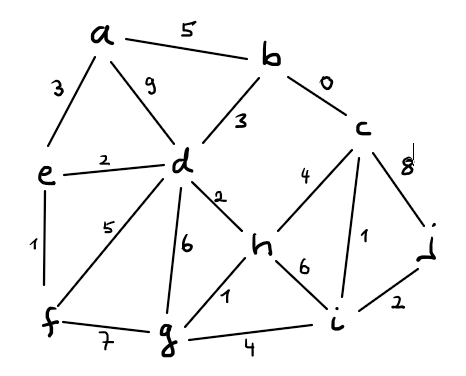
\includegraphics[height=6cm]{\pfad/Graphen/Aufgaben/kruskal_02b/kruskal_02b.png}
\begin{solutionbox}{4cm}
\begin{lstlisting}
b-c, c-i, e-f, g-h, d-e, d-h, i-j, a-e, b-d, Gesamtkosten:  15
\end{lstlisting}

\end{solutionbox}
